

\chapter{RESULT AND DISCUSSION}

\hspace{0.9cm} \begin{figure}[h!]
	\centering	
	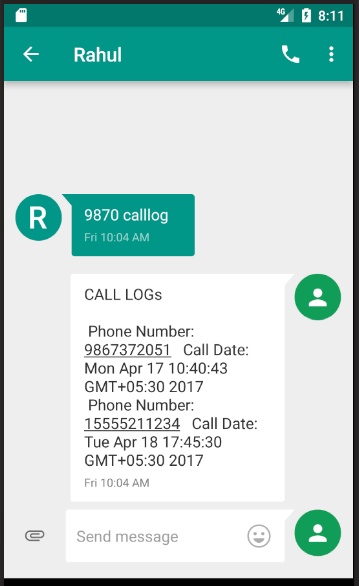
\includegraphics[scale=0.7]{examplecalllog.png} % e.g. insert ./image for image.png in the working directory, adjust scale as necessary
	\caption{Example of calllog retreival}
	\label{fig:9} % insert suitable label, this is used to refer to a fig from within the text as shown above
	
	
\end{figure}

\begin{itemize}
	\item The above image is an example of the message that is generated and sent to the user who sent the commmand "calllog". Our application has satisfied the goals that had been set during the planning phase.
	
	\item The application is suitable for day to day use and most people will find that having this application installed on your phone would be beneficial in the long run. It is better to have the app and not need it, than not having the app and needing it. 
	\item The scope of the application is limited by the system calls which are available to an application in the android eco-system. Some of our ideas on how to add functionality to the application led to a dead end since android simply did not have the necessarily framework to provide the functionality to us.
	
	\item \textbf{Troubleshooting - } We faced a few problems during the course of this project which include but are not restricted to 
		\begin{enumerate}
			\item Different versions of android behave differently which led to a lot of time wastage just in finding out these peculiarities.
			\item The Android Studio IDE is relatively new and as such many implementations avaialable online are for older IDEs like Eclipse.
			\item Many a times the unreliable mobile networks led to the application being unable to function as expected.
			
		\end{enumerate}
	
\end{itemize}

